\documentclass[Kravspecifikation/Kravspec_Main.tex]{subfiles}
\begin{document}

\section{Funktionelle krav}

\subsection{Aktør beskrivelse}
Til at beskrive systemet er der udviklet et aktør kontekst diagram, se figur \ref{fig:Actor-context}.
\begin{figure}[H]
    \centering
    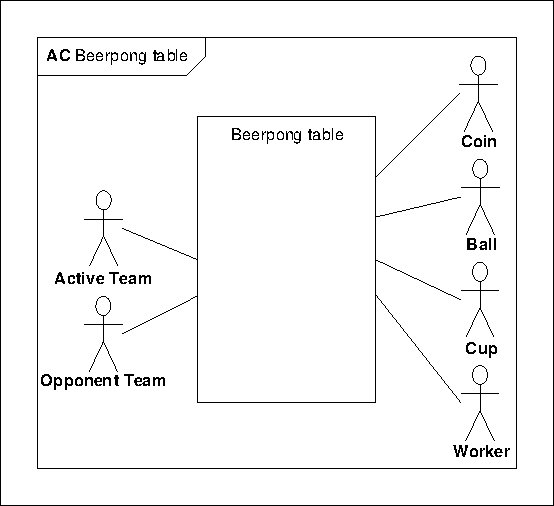
\includegraphics[width=0.8\textwidth,trim={0.24in 0.24in 0.24in 0.24in},clip, page=1]{Kravspecifikation/Funktionelle_krav/graphics_funktionel/Krav-spec-diagrammer.pdf}
    \caption{Aktør kontekst diagram for systemet}
    \label{fig:Actor-context}
\end{figure}

\subsubsection{Active Team}
\begin{table}[H]
    \centering
    \begin{tabular}{|L{0.35\textwidth}|L{0.65\textwidth}|}
        \hline
        \textbf{Aktør navn} & Active Team \\ \hline
        \textbf{Alternativ referencer} & Aktiv hold og Aktiv bruger \\ \hline
        \textbf{Type} & Primær \\ \hline
        \textbf{Beskrivelse} & Er et af holdene til spillet (Beer Pong). Når spillet er i \textbf{\textit{opstart}} skal denne aktør sætte spillet op, som beskrevet i tabel \ref{tab:UC1}. Når spillet er \textbf{\textit{i gang}} er denne aktør det hold som har \textbf{\textit{turen}}, som beskrevet i afsnit \ref{sec:rules}. De to hold der spiller spillet skiftes at være denne aktør \\ \hline
    \end{tabular}
    \caption{Aktør beskrivelse for Active Team}
    \label{tab:ActiveUserBeskrivelse}
\end{table}

\subsubsection{Opponent Team}
\begin{table}[H]
    \centering
    \begin{tabular}{|L{0.35\textwidth}|L{0.65\textwidth}|}
        \hline
        \textbf{Aktør navn} &  Opponent Team\\ \hline
        \textbf{Alternativ referencer} &  Modstander hold, Modstander og Opponent\\ \hline
        \textbf{Type} & Sekundær (UC1 og UC2) og Primær (UC3) \\ \hline
        \textbf{Beskrivelse} & Er det hold i spillet (Beer pong) som ikke er det aktive hold. Det hold som ikke har \textbf{\textit{turen}}. De to hold der spiller spillet skiftes at være denne aktør\\ \hline
    \end{tabular}
    \caption{Aktør beskrivelse for Opponent Team}
    \label{tab:OppponentTeamBeskrivelse}
\end{table}

\subsubsection{Coin}
\begin{table}[H]
    \centering
    \begin{tabular}{|L{0.35\textwidth}|L{0.65\textwidth}|}
        \hline
        \textbf{Aktør navn} & Coin \\ \hline
        \textbf{Alternativ referencer} & Mønt. \\ \hline
        \textbf{Type} &  Sekundær \\ \hline
        \textbf{Beskrivelse} & Er en mønt som skal indsættes i systemet, og returneres afhængig af hvilken mønt det er og systemets tilstand. \\ \hline
    \end{tabular}
    \caption{Aktør beskrivelse for Coin}
    \label{tab:CoinBeskrivelse}
\end{table}

\subsubsection{Ball}
\begin{table}[H]
    \centering
    \begin{tabular}{|L{0.35\textwidth}|L{0.65\textwidth}|}
        \hline
        \textbf{Aktør navn} & Ball \\ \hline
        \textbf{Alternativ referencer} & Bold og Bordtennisbold \\ \hline
        \textbf{Type} & Sekundær \\ \hline
        \textbf{Beskrivelse} & Denne aktør er en bordtennisbold som bruges til at spille spillet (Beer Pong), se afsnit \ref{sec:rules}. Systemet skal også håndtere flere bolde, da det skal dispensere bolde i \textbf{\textit{opstart}}.\\ \hline
    \end{tabular}
    \caption{Aktør beskrivelse for Ball}
    \label{tab:BallBeskrivelse}
\end{table}

\subsubsection{Cup}
\begin{table}[H]
    \centering
    \begin{tabular}{|L{0.35\textwidth}|L{0.65\textwidth}|}
        \hline
        \textbf{Aktør navn} &  Cup\\ \hline
        \textbf{Alternativ referencer} &  Kop og plastik kop\\ \hline
        \textbf{Type} & Sekundær \\ \hline
        \textbf{Beskrivelse} & Denne aktør er en kop. De to hold prøver at ramme i en kop med en bold. Systemet skal registrere om koppen er i en kopholder eller ej.  \\ \hline
    \end{tabular}
    \caption{Aktør beskrivelse for Cup}
    \label{tab:CupBeskrivelse}
\end{table}

\subsubsection{Worker}
\begin{table}[H]
    \centering
    \begin{tabular}{|L{0.35\textwidth}|L{0.65\textwidth}|}
        \hline
        \textbf{Aktør navn} & Worker \\ \hline
        \textbf{Alternativ referencer} & Servicemedarbejder og arbejder \\ \hline
        \textbf{Type} & Sekundær\\ \hline
        \textbf{Beskrivelse} & Denne aktør er en medarbejder for ejeren af systemet. Har til opgave at vedligeholde systemet, dvs. at der skal fyldes bolde i systemet\\ \hline
    \end{tabular}
    \caption{Aktør beskrivelse for Worker}
    \label{tab:WorkerBeskrivelse}
\end{table}


\subsection{Use Case Diagram}
Der benyttes use cases til at beskrive de funktionelle krav. Der er derfor lavet use case diagrammet som kan ses på figur \ref{fig:Use_case}.
\begin{figure}[H]
    \centering
    \includegraphics[width=0.8\textwidth,trim={0.24in 0.24in 0.24in 0.24in},clip, page=2]{Kravspecifikation/Funktionelle_krav/graphics_funktionel/Krav-spec-diagrammer.pdf}
    \caption{Use Case diagram for systemet}
    \label{fig:Use_case}
\end{figure}
Da Der benyttes engelske navne i diagrammer men danske i tekst, er der på tabel \ref{tab:uc_translation} beskrevet de danske navne.

\begin{table}[H]
    \centering
    \begin{tabular}{|L{0.35\textwidth}|L{0.35\textwidth}|}
        \hline
        \textbf{Engelsk} & \textbf{Dansk} \\ \hline
        UC1: Start game & UC1: Start spil \\ \hline
        UC2: Play turn & UC2: Spil tur \\ \hline
        UC3: End game & UC3: Spil slut \\ \hline
        UC4: Refill balls & UC4: Påfyldning af bolde \\ \hline
    \end{tabular}
    \caption{Oversættelse af Use Case navne til dansk}
    \label{tab:uc_translation}
\end{table}

\newpage

\subfile{Kravspecifikation/Funktionelle_krav/Use_cases/UC1-Startspil.tex}
\newpage
\subfile{Kravspecifikation/Funktionelle_krav/Use_cases/UC2-Flytkop.tex}
\newpage
\subfile{Kravspecifikation/Funktionelle_krav/Use_cases/UC3-Spilslut.tex}
\newpage
\subfile{Kravspecifikation/Funktionelle_krav/Use_cases/UC4-opfyldbolde.tex}
\newpage

\end{document}

